\chapter{Informacje nieprawdziwe w dobie internetu}
Pojęcie ``Fake news'' odnosi się do 
informacji, które pomimo że nie posiadają pokrycia z rzeczywistością są 
przedstawiane jako prawdziwe w mediach takich jak np.: wiadomości, artykuły, 
portale społecznościowe itd.. 
Zwrot ten jest neologizmem i w języku angielskim oznacza dosłownie ``Fałszywe wiadomości''
celem wykorzystania takich wiadomości mogą być żarty np.: satyra, jednak najczęsciej 
mają one jedno z dwóch zadań:
\begin{itemize}
    \item oszukać odbiorcę i wpłynąć na jego poglądy w sposób żądany przez autora danej informacji \emph{Propaganda}
    \item namówienie go na zakup czegoś czego w innym przypadku by on nie kupił \emph{Reklama}
\end{itemize} 
Niektóre fałszywe informacje łączą oba cele.

Fake news'y stały się bardzo popularnym zagadnieniem w ostatnich czasach ponieważ
internet a w szczególności media społecznościowe pozwoliły na przekazywanie 
informacji z niespotykaną wcześniej prędkością dzięki czemu rozprzestrzenianie 
dezinformacji stało się zadaniem stosunkowo prostym.

Zagadnienie to zyskało ogromny rozgłos podczas kampanii wyborczej oraz
prezydentury Donalda Trumpa, który zasłynął z częstego wykorzystywania 
tego zwrotu podczas wywiadów debat oraz wypowiedzi na mediach społecznościowych
tj. Twitter.
Do roku 2020 pojęcie ``Fake News'' zostało umieszczone w słownikach języka angielskiego
takich jak ``Oxford English Dictionary'', ``Macmillan Dictionary''.
\begin{figure}[h!]
    \centering
    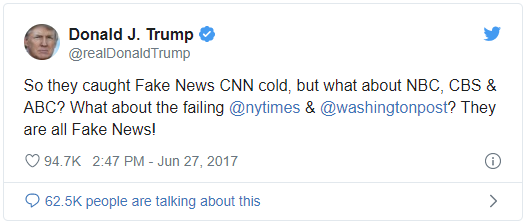
\includegraphics[width=0.7\textwidth]{./Img/Trump-Fake-News.png}
    \caption{Post udostępniony przez Donalda Trumpa na portalu Twitter}
\end{figure}

Według założonego przez dziewięć organizacji w skład których wchodzą 
Google, Facebook oraz Twitter projektu ``First Draft News''
możemy wyróżnić siedem typów Fake Newsów:
\begin{enumerate}
    \item Satyra bądź parodia
    \item Fałszywe połączenie
    \item Myląca zawartość
    \item Fałszywy kontekst
    \item Oszukana zawartość
    \item Zmanipulowana zawartość
    \item Sfabrykowana zawartość
\end{enumerate}
Jak podaje słownik ``Merriam Webster'' po raz pierwszy wykorzystano zwrot
``Fake news'' w roku 1890.


Jednym z najsłynniejszych typów fake newsów jest propaganda, czyli według 
definicji ``technika sterowania poglądami i zachowaniami ludzi polegająca na 
celowym, natarczywym, połączonym z manipulacją oddziaływaniu na zbiorowość''
pomimo iż najczęsciej propaganda ma charakter polityczny nie jest to jedyne 
jej zastosowanie. Najstarszym przykładem pisemnej propagandy są opisy podbojów
Dariusza Wielkiego datowane na rok 515 p.n.e. Od tego czasu w historii ludzkości
można znaleźć wiele przypadków wykorzystania tego typu dezinformacji w takich krajach
jak Starożytny Rzym, Niemcy podczas drugiej wojny światowej a nawet w dzisiejszych 
czasach Korea Północna.
Propagandę można podzielić na 3 różne typy:
\begin{enumerate}
    \item Biała propaganda - źródło pochodzenia informacji jest prawdziwe i podane
    \item Szara propaganda - źródło pochodzenia informacji jest dla odbiorcy nieznane i może się on jedynie domyślać
    \item Czarna propaganda - źródło pochodzenia informacji jest umyślnie sfałszowane w celu wyrządzenia szkody 
\end{enumerate}


% historia fake newsow 
\section{Sposoby rozprzestrzeniania fałszywych informacji}
Wraz ze zmianami w sposobach rozprzestrzeniania informacji na świecie zmieniało się
także podejście do tworzenia fake newsów w odpowiedni sposób oszukujących osoby do których 
były one skierowane. 

\subsection{Gazety}
Wykorzystanie fake newsów w gazetach miało głownie na celu przyciągnąć uwage a co za 
tym idzie zwiększyć sprzedaż danej gazety. Stało się to na tyle popularne że spowodowało
narodziny nowego pojęcia ``żółtej prasy'' była to prasa starająca się z całych sił zwrocić
uwagę przechodnia poświęcając swoją wiarygodność poprzez zawarcie w nagłowkach w pełni lub
częściowo nieprawdziwych wiadomości. Dziennikarz Frank Luther Mott wyróżnia 5 cech charakteryzujących
żółtą prasę:
\begin{itemize}
    \item Napisane dużą czcionką straszące nagłówki na temat mniej ważnych wydarzeń
    \item Nadmierna ilość zdjęć i rysunków
    \item Zawarcie sfałszowanych wywiadów, mylących nagłowków, pseudonauki oraz nieprawdziwych informacji od ludzi podających się za ekspertów
    \item Dodanie w pełni kolorowych dodatków do gazet w niedzielę
    \item Stawianie siebie jako słabszego w walce przeciwko systemowi
\end{itemize}
\begin{figure}[h!]
    \centering
    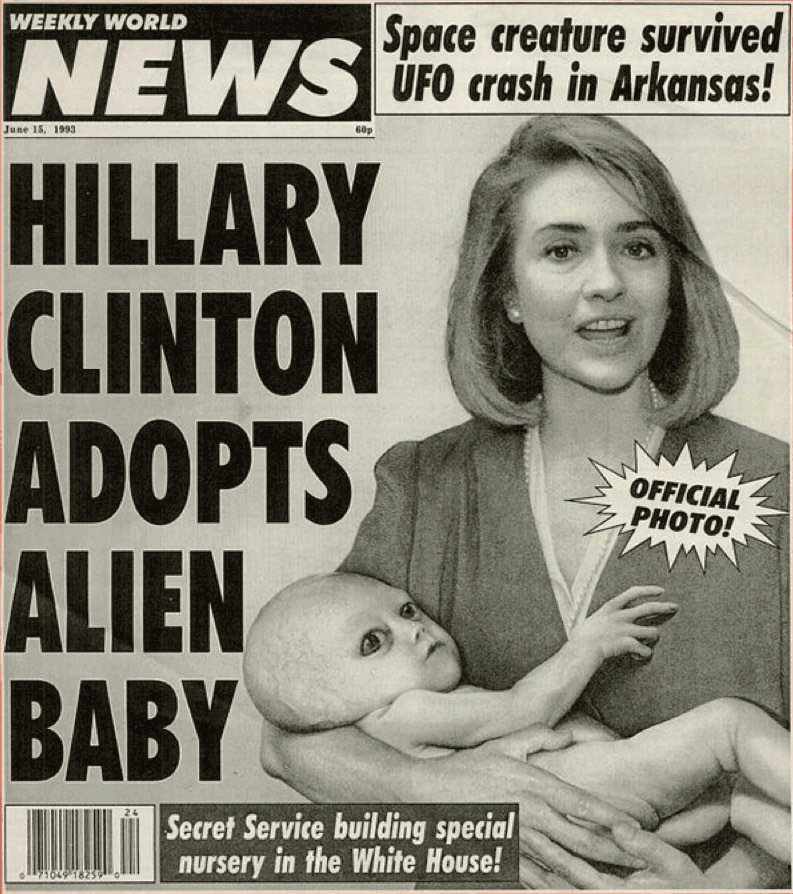
\includegraphics[width=0.5\textwidth]{./Img/fake-newspaper.jpg}
    \caption{Przykład żółtej prasy z roku 1993}
\end{figure}

\subsection{Telewizja}

\subsection{Internet}
\section{Deep fake}

\section{Sposoby ochrony przed nieprawdziwymi informacjami}
